%Chapter describing the mimetic process
\chapter{Mimicry}

\begin{quote}
``It is not the strongest of the species that survives, nor the most intelligent that survives. It is the one that is the most adaptable to change. - Charles Darwin"
\end{quote}

\section{History}
Henry W. Bates first published in 1862 his findings about the similarities and dissimilarities between Heliconiinae and Ithomiinae butterflies, after 10 years of research in the Brazilian rain forest. For the next hundred years, it simulated heated discussion among all groups of people, scientists, philosophers, theologians, teachers and amateur naturalists. Bates collected ninety-four pieces of butterfly. He grouped them according to their similar appearance. He found butterflies having similar appearance, exhibiting morphological features which point to completely different species even families. Out of the ninety four species sixty seven are now classified as Ithomiinae, while twenty seven of them are Heliconiinae.

\section{Batesian Mimicry}
Even though Heliconiids are conspicuously colored, they are extremely abundant. They were also slow in mobility. Still predators in the surrounding area, mostly insectivorous birds do not prey on them, because of their inedible and unpalatable nature. Also because of this phenomenon other edible and palatable species such as ithomiinae and pieridae, pretend to be heliconiids and thus enjoy protection.

Repulsive animals, such as heliconiids are very conspicuously colored. Having this noticeable property, they are easily recalled by predators. Their wing pattern works as a warning to them. Once a predator has the knowledge of their inedible and unpalatable property, they would probably never attempt to try it again. As this is true, if any organism within close family and species, but being edible and having a deceptive resemblance to those conspicuously colored species will be avoided by the predators. Wickler \cite{wickler1986} expresses,
\begin{quote}
``Such unpalatable appearing and yet edible animals thus possess a false warning pattern, they 'act a part'. An actor is a mime, and so the representation of a false warning pattern was called \textit{mimicry}. Since Bates was the first to point out this phenomenon, it has received the name \textit{Batesian Mimicry} in his honor."
\end{quote}
In general, the animal which is avoided by predator for unpalatable behavior is called the \textbf{model} and the imitating animal is called the \textbf{mimic}.

\begin{figure}[H]
	\centering
	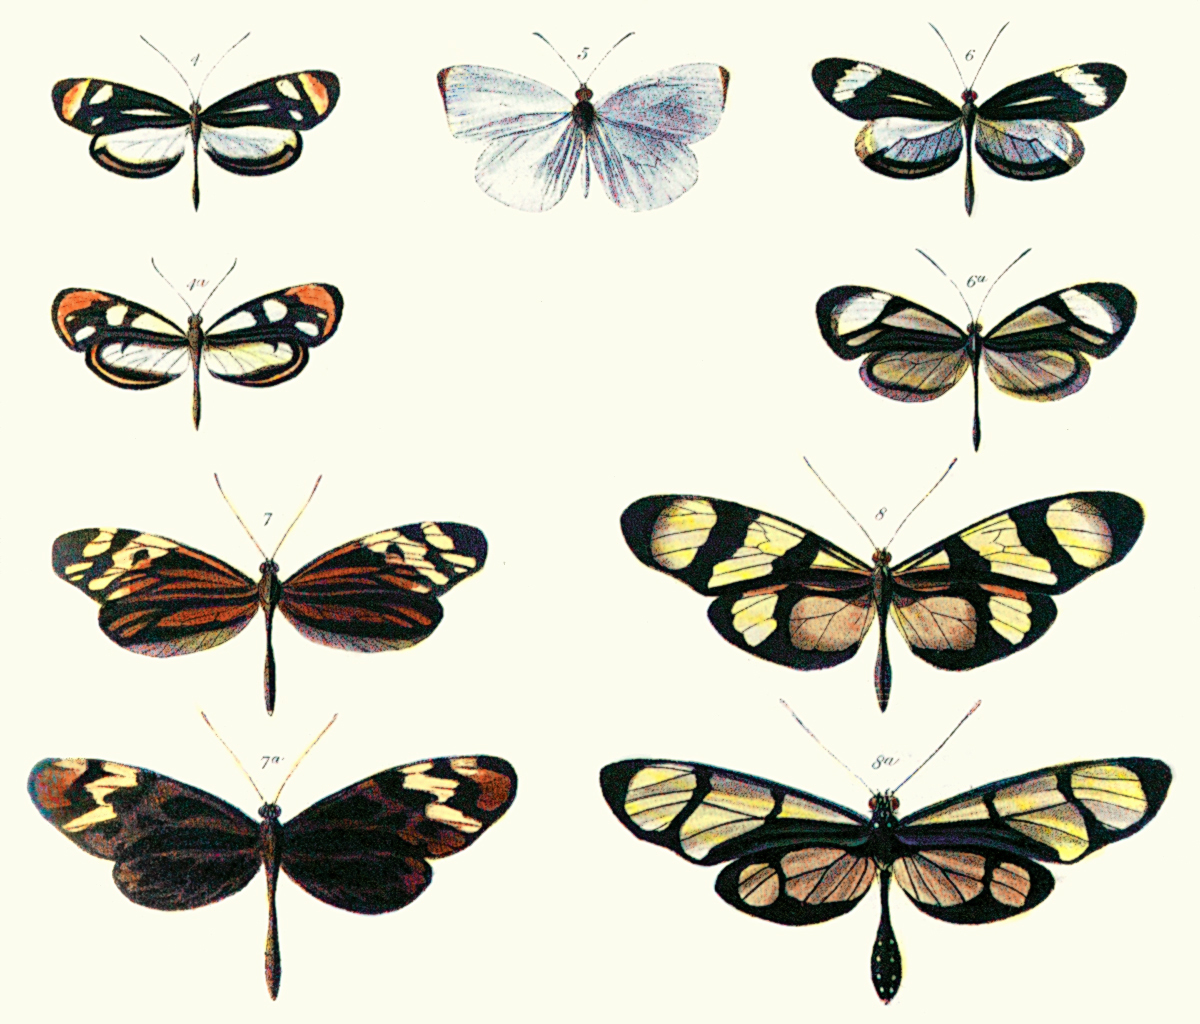
\includegraphics[scale=1]{images/Batesplate_ArM}
	\caption{Plate from Bates (1862) illustrating Batesian mimicry between Dismorphia species (top row, third row) and various Ithomiini (Nymphalidae) (second row, bottom row). \cite{bates1862}}
	\label{fig:plot-2-prey}
\end{figure}

\subsection{Definitions of Mimicry}
The definition of mimicry provided by Bates is quite restricted and is similar to the following

\begin{quote}
``resemblance in external appearance, shapes and colours between members of widely distinct families."
\end{quote}

The following more sophisticated definition was provided at the international Zoological Congress in Washington, 1963,

\begin{quote}
``Mimicry is the close resemblance of one organism to another which, because it is unpalatable and conspicuous, is recognized and avoided by some predators at some times."
\end{quote}

The best known defintion of mimicry quoted to the present day, are those given by Wallace and listed in Poulton's \textit{The color of animals, their meaning and use} \cite{poulton1890colours}. The clauses are presented in the following:

\begin{itemize}
	\item ``that the imitative species occur in the same area and occupy the same station as the immitated". This increases the probability that a predator will affect both parties concerned. Neverthless, the model could live in Africa and the mimic in Europe, or vice versa, if the deceptive predator were a migratory bird.
	\item ``that the imitators are always the more defenceless". It will be seen later on in the discussion of Mertensian mimicry among coral snakes that the more offensive party may occasionally be the mimic. 
	\item ``that the imitators are always less numerous in individuals". What is meant here is that the deceived animal should encounter the mimic less often than the model. This is true when the deceived animal must learn to recognize model and mimic and when positive and negetive experiences carry equal weight. But it is known from various learning experiments that when an animal has learn about warning coloration, negetive experiences or punishment stimuli (such as iedibility) can have a stronger and more lasting effect than positive experiences. Accordingly it should be expected that there would be an excess of mimics over models in proportion to the degree of predominance of negative experiences over positive onces. When the deceptive animal possesses an innate reaction to the model the number of mimics can be virtually unlimited. 
	\item ``that the imitators differ from the bulk of their allies". When this condition applies, our attention is of course most easily attracted. The most remarkable cases of mimicry are those where close relatives form divergent models. It is neverthless highly possible that groups of closely related species may be similar mimics of the same model. Of course, it must always be remembered that species can look very different from their relatives because of adaptations which have nothing to do with mimicry. 
	\item ``that the imitation, however minute, is external and visible only, never extending to internal charecters or to such as do not affect the external appearance." This criteria, like the previous one is aimed at defining mimmicry as a special adaptation. But if one of two closely related species both of which are posinous and possess similar warning coloration, should secondarily lose its poisonous qualities, it would become a mimic and yet resemble its model in almost all its non-mimetic characters.
\end{itemize}

These five requirements, if fulfilled, indeed increase the probability that any given case of mimicry will be correctly diagnosed. But such supplementary clauses cannot be used as a definition of mimicry in general, though this is unfortunately often attempted. 

\section{Mullerian Mimicry}
Bates was not able to explain some phenomenon of mimicry. Occasionally two inedible unrelated butterfly species are amazingly similar in appearance. An explanation for this was provided by Fritz Muller in 1878. Like Bates, Muller observed and caught butterflies in Brazil. When there are multiple inedible species it is hard for predators to recognize each of them to know which one to consume and which one to avoid. Because of predator's limited memory, all these species still loose their number even after being inedible. So to save this loss, and to prevent more sacrifice of their own kind, inedible species from different family also tend to evolve to have similar appearance. This phenomenon is referred to as Mullerian Mimicry in the name of Fritz Muller.

\section{Formation of Mimicry Rings}

\section{Other form of mimicry}

\section{Conclusion}